\documentclass[border=10pt]{standalone}
\usepackage{tikz}
\usetikzlibrary{decorations.pathmorphing}
\thispagestyle{empty}
\begin{document}
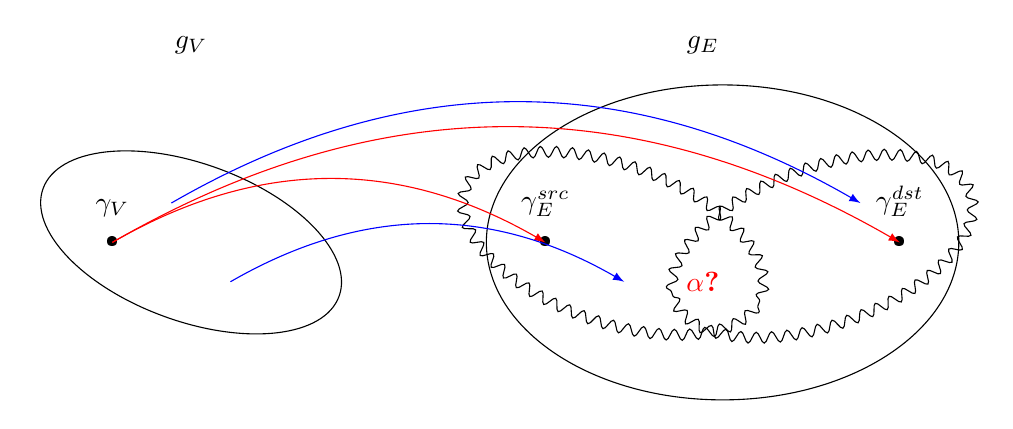
\begin{tikzpicture}
%\draw[help lines] (0,0) grid (10,10);

\draw[rotate around={-20:(-5,1)}] (-5,1) ellipse (2cm and 1cm);
\node[label=above:{$\gamma_V$}] at (-6,1) (vid) {\textbullet};
\node at (-5,3.5) {\textbf{$g_V$}};


\draw (1.75,1) ellipse (3cm and 2cm);
\node at (1.5,3.5) {\textbf{$g_E$}};

\draw[rotate=-20,decoration={snake, amplitude=.7mm, segment length=2mm}, decorate] (0,1) ellipse (2cm and 1cm);
\draw[rotate around={200:(3,1)},decoration={snake, amplitude=.7mm, segment length=2mm}, decorate] (3,1) ellipse (2cm and 1cm);
\node[label=above:{$\gamma_E^{dst}$}] at (4,1) (dst) {\textbullet};
\node[label=above:{$\gamma_E^{src}$}] at (-.5,1) (src) {\textbullet};
\node at (1.5,0.5) {\color{red}\textbf{$\alpha$?}};

\draw[-latex,red] (-6,1) to [bend left] (4,1);
\draw[-latex,red] (-6,1) to [bend left] (-.5,1);
\draw[-latex,blue] (-4.5,.5) to [bend left] (.5,.5);
\draw[-latex,blue] (-5.25,1.5) to [bend left] (3.5,1.5);
\end{tikzpicture}
\end{document}